\section{Introduction}
Main goal: Argue for SC, and \xQ. Present \xQ{} and justify decisions. Demonstrate the performance on `realistic simulations'.

\nisar{can probably borrow text from Matt's RSS paper and Nick's InfoTech paper to help establish the context and motivation for this work...to argue for need for assurances and self-confidence, need to first establish that autonomous systems/robots are here and rely heavily on ML techniques as well as decision-making algorithms to operate under uncertainty...difficult to ensure transparency because same inputs/operating conditions may lead to different behaviors, which in turn affects user trust...lots of work lately on trust in autonomous systems (cite some refs), which relates very closely to question of how to establish transparency and explainability and predictability, etc. for ML systems...key difference is that autonomous systems are to a large extent expected to be self-directed and self-sufficient decision makers -- though, in reality, they must operate within a delegated scope of action and competency (cite Johnson's `Seven Deadly Myths of Autonomous Systems') ... thus the transparency/explainability question in this case is: how does a system know its own limits and convey this to a user/stakeholder? Or, equivalently: how can an autonomous system justify it's ability to accomplish a task? note: they key insight we bring to the table here is that the question of introspection and communication of a machine's own limits is itself a complex problem of meta-reasoning that requires its own set of AI/learning approaches to tackle...leads to idea of algorithmic self-confidence as an assurance...  }

within the scope of FAT* `topics of interest' we fall under the \emph{Transparency} branch. Specifically `Interpretability of ML models', and `Generation of explanations' (although probably more interpretability according to most people's definitions).

withing the scope of the FAT* tracks I believe that we align with:

\begin{enumerate}
    \item Statistics, Machine Learning, and Data Mining
    \item HCI, and Information Visualiation
    \item \ldots possibly something along the lines of empirical studies, as that is what we intend to do
\end{enumerate}

We can choose `archival' or `non-archival'. I think we probably want to do archival, since this is a promising `home' for our research anyway.

\nisar{very important: need a statement of contributions -- why should this audience care about this work? what is the intellectual contribution? (would be good to see other papers from previous year's proceedings to see examples)}

\subsection{Proposed outline:}

\begin{itemize}
    \item Motivation---why MDPs, why meta-analysis, why self-confidence? \nisar{should add in some background about autonomous systems concepts that are relevant for this audience to pick up key ideas...}
    \item Related work---quickly review some related work in the area \nisar{what other ideas specifically should be mentioned?}
    \item Approach---desiderata, Hellinger distance, etc
    \item Results/Discussion---Illustrative example, and theoretical example
    \item Conclusions/Future Work---restate purpose of SC, and particularly \xQ. Discuss continuing efforts to quantify effects with human-involved experiments. Further development of \xH, \xI, and \xM.
\end{itemize}

\subsection{Related Work}
    Discuss related work such as

    WHY DO WE USE MDPS? THEY ARE A GOOD PLACE TO START FROM, AND ARE CONNECTED TO MANY OTHER LEARNING APPROACHES (REINFORCEMENT, INVERSE REINFORCEMENT, \ldots)

    Reinforcement learning is finding a policy when transitions, and states are unknown. Basically learn policy and model simultaneously.

    inverse RL is learning a reward function by observing a policy.

\subsection{Factorized Machine Self-Confidence}
    \begin{figure*}[tbp]
        \centering
        \includegraphics[width=0.65\linewidth]{Figures/SC_flowchart.pdf}
        \caption{Factorized Machine Self-Confidence}
        \label{fig:famsec}
    \end{figure*}

    Several definitions of self-confidence have been proposed in recent works. Much of this work is reviewed in \cite{Israelsen2017-ym}, where self-confidence is identified as an explicit assurance in a human-autonomy trust relationship. According to \cite{Sweet2016-tz} the four views on self-confidence are the \textit{anthropomorphic view}, the \textit{uncertainty view}, the \textit{experiential view}, and the \textit{stability view}. The anthropomorphic view defines self-confidence to be similar to how humans express self-confidence, while the experiential view expresses self-confidence based on past experience. The uncertainty view simply defines self-confidence to be the probability of success or failure, and the stability view defines self-confidence to be the sensitivity of the probability of success to uncertainty. All of these views seem to reflect different parts of a more general concept: understanding an autonomy's ability to do a specific task. This leads to the following definition of self-confidence.

    We define self-confidence to be: \textbf{An agent's perceived ability to achieve assigned goals (within a defined region of autonomous behavior) after accounting for (1) uncertainties in its knowledge of the world, (2) uncertainties of its own state, and (3) uncertainties about its reasoning process and execution abilities.}

    The formal definition of self-confidence we use is from \cite{Aitken2016-cv}, wherein five factors that compose self confidence are defined. They are: \nisar{can add some more detail from proposals...}

        \begin{itemize}
            \item [\xH{}:] \textbf{Past Performance}---how well has autonomy done in similar circumstances?
            \item [\xI{}:] \textbf{Command Interpretation}---are autonomy and user `on the same page'?
            \item [\xM{}:] \textbf{Model Validity}---How well does autonomy's model reflect reality?
            \item [\xP{}:] \textbf{Predicted Outcome Assessment}---How favorable is the distribution of predicted outcomes?
            \item [\xQ{}:] \textbf{Solver Quality}---How well can the solver use the model to generate policies/plans?
        \end{itemize}

    Outcome assessment has been previously defined in \cite{Aitken2016-cv}, but has not yet been evaluated as an effective assurance as per the guidelines laid out in the work on assurances. Solver Quality is a metric that is, as yet, un-explored.

\subsection{Solver Quality (\xQ)} \label{sec:SQ}
    The main aim of \xQ{} is to indicate how solver \solve{} will perform on a given (possibly un-encountered) task \task{}. The desiderata are:

    \begin{enumerate}[label=\textbf{D\arabic*}]
        \item enable comparison across solver classes \label{itm:d1}
        \item reflect competence of solver \solve{} for task \task{} \label{itm:d2}
        \item extend to unseen tasks \label{itm:d3}
    \end{enumerate}

    Solvers of all classes are similar in that they operate on a specified problem, and have defined solver parameters that govern their behavior, in order to produce a policy $\pi$ that is a mapping from states to actions. In order to evaluate the quality of some solver on a given task \task, we propose comparing the policy \policy{} produced by \solver{} on \task{} to a `ground truth' policy $\pi^*$. This raises the question of how to compare policies. There are a few different approaches that present themselves:

    \begin{enumerate}
        \item Compare utilities at each state \label{itm:i1}
        \begin{itemize}
            \item Merits: Evaluates whether states have similar utilities, quick to calculate
            \item Demerits: Does not apply to solvers that represent different amounts of the state-action space (i.e. exact versus approximate solvers), or to solvers that may represent the state-action space differently (i.e. meta-solvers). This approach does not satisfy \ref{itm:d1}.
        \end{itemize} 
        \item Compare `coverage' of the policy \label{itm:i2}
        \begin{itemize}
            \item Merits: Evaluates how `thorough' the policy is, quick to calculate
            \item Demerits: Does not meet \ref{itm:d1} because not all policies will have the same coverage by design. Also high coverage does not imply a `good' solution
        \end{itemize}
        \item Compare the reward distribution of given policies \label{itm:i3}
        \begin{itemize}
            \item Merits: Meets \ref{itm:d1}
            \item Demerits: Expensive to calculate the reward distribution via many simulations
        \end{itemize}
    \end{enumerate}
    
    Given the requirement to operate on different classes of solvers the \xQ{} metric must operate only on information available to all classes of solvers. Namely, \xQ{} should take as inputs: the problem definition, and solver parameters. The result should be some metric based on the resulting policy \policy. This approach is inspired by \cite{Leyton-Brown2009-yr} who were able to use `Empirical Hardness Models' (EHMs) to predict the empirical runtime performance of an algorithm on a problem with given features. Figure~\ref{fig:SQ_flowchart} illustrates how this might work for \xQ{} as an assurance.

    A model is trained in order to predict sufficient statistics of the trusted, or reference, solver \solvestar{} on different (but similar) tasks. The solver quality metric compares the reward distribution of the candidate solver to the predicted distribution of the trusted solver for a task.

    \begin{figure}[tbp]
        \centering
        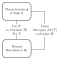
\includegraphics[width=0.7\linewidth]{Figures/SQ_train.png}
        \caption{Figure displaying that \surrogate{} is use to predict a distribution  \rwdstariapprox{} that matches the first and second moments of \rwdstari}
        \label{fig:sq_train}
    \end{figure}%

    \begin{figure}[tbp]
        \centering
        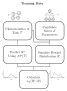
\includegraphics[width=0.6\linewidth]{Figures/SQ_test.png}
        \caption{During testing \surrogate{} is used to predict \rwdstarapprox{}, \xQ{} is then calculated using \rwd{}.}
        \label{fig:sq_train}
    \end{figure}
